
\documentclass[a4paper,11pt,twosideX,onefignum,onetabnum]{siamart190516}


\externaldocument{ex_article}
\usepackage{graphicx}
\usepackage{amsmath,amsfonts,amssymb,float}
\usepackage[utf8]{inputenc}
\usepackage[T1]{fontenc}
\usepackage{lscape}
\usepackage{boldline,multirow,tabularx,colortbl,diagbox,makecell,fancybox}
\usepackage{pdfpages}
\usepackage{amsfonts,amssymb,amsmath,mathrsfs,array}
\usepackage{pgf,tikz,xcolor}
\usetikzlibrary{calc,positioning,shapes.geometric,shapes.symbols,shapes.misc, fit, shapes, arrows, arrows.meta,fadings,through}
\usepackage[top=2cm, bottom=2cm, left=2cm, right=2cm]{geometry}
\usepackage{hyperref}
\usepackage{titlesec}
\usepackage{eurosym}
\usepackage[english]{babel}
\usepackage{graphicx,subcaption}
\usepackage{adjustbox}
\renewcommand{\thefootnote}{(\texttt{\tiny\arabic{footnote}})}




\begin{document}
\title{Estimating river discharge by learning processes in spatial hydrology}
\author{Sébastien Castets\thanks{student at INSA Toulouse, sbcastets@gmail.com}\and Quentin Douzery \thanks{student at INSA Toulouse, qdouzery@free.fr }\and Elisa Escanez \thanks{student at INSA Toulouse, elisa.escanez@g-mail.fr} }
%\thanks{, , }


\maketitle
\section*{Abstract.}

Managing water consumption and predicting flood risk are crucial issues which needs to better understand river flow on a global scale. Currently, data on rivers is poorly distributed geographically and temporally. Thus, in 2022, NASA and CNES will launch a satellite to collect altimetric data on rivers to reinforce the databases. However, a lack of knowledge exists in physical models which predict rivers flow, there is a bias on its value. We aim to use neural networks to reduce the bias and thus to obtain more accurate predictions. We performed an advanced statistical analysis on data to highlight the main parameters related to river discharge, and we built Artificial Neural Networks and Long Short-Term Memory Networks to estimate river discharge. We obtained satisfying results when the amount of data was sufficient, as the bias disappeared, but the predictions were not as high as expected when the dataset size was small. We conclude that our two different neural networks have two different aims, as an ANN can predict the river discharge for any river and the LSTM just for a particular river, and that the amount of data is the crucial point of the issue of the river discharge estimation.



\section{Introduction.}

The prediction of water variation is an important issue. The crucial point is to predict river discharge on a global scale for two main reasons.  In some countries or regions, water is a limited resource, and it often depends on the season. On the contrary, in others regions, water can cause disasters and environmental damage such as floods. Therefore, water forecasting is important to manage water consumption in agricultural or industrial sectors, in people's daily lives, or to evacuate a population in case of an imminent threat. In addition to the environmental issues, rivers are at the center of geopolitical tensions. According to the United Nations, "2 billion people live in countries experiencing high water stress" (UN, 2019 \cite{ONU}). From the water stress results a higher water demanding than the available resources. 

Although the water stress is rising, there are still few data on rivers : the data is poorly distributed geographically and temporally (Matt Fry, 2019 \cite{insitudata}). Moreover, only few countries share these resources. Scientists struggles to estimate the space-time water variation of rivers due to theses reasons (Monnier, 2021 \cite{conf_monnier}). They need to know the exact bathymetry value, the friction coefficient and the potential lateral flux to compute a river flow model (Nils Reidar B. Olsen, 2004 \cite{courshydro}). But these data are very often unknown because of the complexity to measure them.

NASA and CNES created Surface Water Ocean Topography (SWOT) mission (NASA, \cite{NASA}). In April 2022, the first satellite studying only water surfaces (rivers and oceans) will be launched. It will collect altimetric data on rivers wider than 50 meters. The SWOT instrument will observe rivers surface topography and measure how water bodies change over time. Through the observations, it will measure the elevation and the width of rivers. The data collection will last for 3 years with 21 days repeat cycle and will cover the majority of the earth.

Given the SWOT data, hydrologists will face an inverse and ill-posed problem. Using altimetric data, they cannot find exactly the river flow. They need an additional data such as the incoming river flow or the unobserved cross-sectional flow area. And the satellite will not be able to capture this data.\newline

However, scientists manage to predict well water variations, but it exists a potential bias. This bias is due to ungauged rivers where we do not have additional data. We aim to estimate river flow using neural networks without knowing the bathymetry. The objective is to have an estimation without bias.\newline

In this paper, we use two different types of neural networks algorithms. The first one is an Artificial Neural Network (ANN), and the second one a Long Short-Term Memory (LSTM) network, which has feedback connections. This feature is the major point which permits us to reduce the bias.

First, a brief overview of our two datasets HydroSwot and PEPSI and a statistical analysis will be given. After detailing the methods, we will highlight the most important variables and define classes.  Second, we will concentrate on neural networks setup and theory, especially Artificial Neural Networks and Long Short-Term Memory Networks. Third, we will show how neural networks permit to predict river discharge. We will end this paper with a discussion about the different ways to improve the models we computed.


\newpage
\section{Dataset analysis}

\subsection{Dataset presentation and modifications}

\subsubsection{Dataset presentation.}

We focus on two datasets. The first one is PEPSI, a compilation of synthetic flow observations generated from outputs of various hydraulic flow models. This dataset is composed of 55525 observations from 29 rivers worldwide, with 21 explanatory variables for each of them. The second dataset, HydroSwot is generated from observations -- from 153 rivers -- taken in-situ in North America. It contains 16638 observations with 41 explanatory variables. Table \ref{tab:varaibles} describes the explanatory variables contained in both datasets, and that we use for the statistic analysis.


\begin{table}[H]
    \centering
    \begin{tabular}{|c|c|c|c|}
    \hline
        Variable & Description & HydroSwot & PEPSI  \\ \hline \hline
        river &  river name & X & X \\ \hline
        site\_no & site number & X & \\ \hline
        day & simulation day & & X \\ \hline
        reach & reach index & &X \\ \hline
        reach\_length & length of the reach & & X \\ \hline 
        flowacc & flow accumulation, i.e. size of the upstream watershed & X & X \\ \hline
        height & free surface height & X & X \\ \hline 
        dH & water depth above unobserved flow & X & \\ \hline
        W &  free surface top width & X & X \\ \hline
        S & free surface slope  &  & X \\ \hline
        Sdem & terrain slope & X & \\ \hline
        K & Strickler value & & X \\ \hline
        Fr & Froude number & & X \\ \hline
        \alpha, \beta & Manning-Strickler coefficients & & X \\ \hline 
        A & cross-section flow area & & X \\ \hline 
        dA & cross-sectional flow area above A0 & X & X \\ \hline
        A0 & unobserved cross-sectional flow area & X & X\\ \hline
        Abar & mean cross-sectional flow area  data & X & X\\ \hline
        Amed & median cross-sectional flow area  data & X & \\ \hline
        U & flow velocity & X & X\\ \hline
        Q & discharge & X & X \\ \hline
        PA & mean annual precipitation & X & \\ \hline
        TA & mean annual temperature & X & \\ \hline
        sinuosity & sinuosity & & X \\ \hline 
        meandwave & meandering wavelenght & & X \\ \hline 
        Sand, salt, ... & floor composition & X &X \\ \hline 
        lon, lat & localisation & X & X \\ \hline 
        LC1, LC2, ... & vegetation information & X & \\ \hline 
        
    \end{tabular}
    \caption{Explanatory variables of HydroSwot and PEPSI datasets}
    \label{tab:varaibles}
\end{table}
\underline{Remark:} the values of the river discharge $Q$ have an uncertainty of 20\%. 


\subsubsection{Dataset modifications.\label{section212}}

First, we clean our datasets. We delete all observations with $NaN$ values, i.e. missing values. In the HydroSwot dataset, we can find different names for the same river because of text processing when creating the data. We update the names to have each river with a single name and make easier the analysis. We obtain 134 rivers.

The satellite does not detect small rivers with a width less than $80m$. Thus, we delete observations with a width under $80m$. We also remove observations with a river discharge under $100 m^3/s$ because we assume they are too precise observations, and so they do not have a real meaning.

We remove the calculations of base streamflow, and the different mean discharge quantile from the HydroSwot dataset. We also remove the flow velocity $U$ in the two datasets, because $U$ is linearly linked to $Q$ according to the following equation : $Q = AU$.\newline

Finally, we obtain a dataset with 29 rivers, 51269 observations, and 20 variables for PEPSI, and a dataset with 134 rivers, 11851 observations, and 21 variables for HydroSwot.
        
Due to previous modifications, we obtain only 1 observation for 8 sites in the HydroSwot dataset. We cannot use these data because the variables $dA$ and $dH$ are calculated by differences, so we must have at least 2 observations to give them meaning. Hence, we remove these 8 observations. To conclude, we lose 29\% of data in the HydroSwot dataset and 8\% in the PEPSI dataset.

\subsection{Statistical methods}

\subsubsection{Correlation matrix.}

We seek to determine which variables are related. 

The correlation is the relationship between two random quantitative variables which explains how they are linearly related. It is defined by :
\begin{equation}
    Cor(\underline{x},\underline{y}) = \frac{Cov(\underline{x},\underline{y})}{\sqrt{Var(\underline{x})Var(\underline{y})}}
\end{equation}
where \underline{x} and \underline{y} denote the samples of the two variables, $Cov$ the covariance between them, and $Var$ their respective variance. The correlation varies between $-1$ when the variables vary in strong opposite directions, and $1$ when they vary exactly in the same direction. Here, we use a correlation matrix to easily summarise all the correlations between all variables : one cell of the matrix represents the correlation between the row variable and the column one. Thus, the diagonal is full of $1$s, as it represents the correlation between a variable and itself.\newline

\subsubsection{Principal Component Analysis.}

The goal of  a Principal Component Analysis (PCA) (Wikistat, 2016 \cite{ACP}) is to reduce the large shape of our problem by gathering our variables within metavariables to analyse our data more easily. The first step consists in a normalization of the data because of the different scales (understand units) of our variables. Then, we compute linear combinations of our initial variables. One linear combination represents one principal component or direction. The aim is to find which direction maximises the amount of variance of the data, i.e. the direction that captures most information of the data. 

Let $\Sigma$ be the covariance matrix associated to the normalized data. Computing the principal component involves determining the eigenvector $a_1$ associated to the largest eigenvalue of $\Sigma$ denoted as $\lambda_1$, i.e. to solve the following equation :
\begin{equation}
    \Sigma a_1 = \lambda_1 a_1
\end{equation}
Thus, we get the principal components by order of significance by ranking the eigenvectors according to the values of their associated eigenvalues. Then, we select the number of axes which is necessary to capture the majority of the information. A well-known rule is to keep the first $n$ components such as the sum of their variances reaches $80\%$ of the total variance.

Finally, we interpret our PCA with two different types of graph. The first one is the loading plot: all the variables of the problem are displayed in the spans formed by each pair of principal components retained. The aim is to find how the initial variables are related with the principal components. The second plot is the score plot, which plots the individuals' coordinates in the the same spans as mentioned above. We then can observe clusters of individuals.

\subsubsection{Clustering by K-means.}

K-means is an unsupervised classification method to define clusters in a dataset. We first have to find the optimal number $k$ of clusters to give to the algorithm. Then, it works as follows.

First, $k$ class centers, called centroids, are randomly initialized. Second, individuals are assigned to the class whose center is closest, according to the chosen distance metric. Here, we use the Euclidean metric. It is defined as follows, for a pair of samples $a$ and $b$ $\in \mathbb{R}^n$:
\begin{equation}
    dist_{euc}(a,b) = \sqrt{\sum^n_{i=1} (a_i - b_i)^2}
\end{equation}

Third, the centers of gravity of each class are computed. Finally, we repeat second and third instructions until the convergence of the algorithm.

One advantage of the K-means algorithm is that we are certain to obtain a convergence of it. Nonetheless, we obtain different classes depending on the random initialization at the beginning. To overcome this problem, the algorithm will be run with different centroid seeds, and the final results will be the best output in terms of inertia.

\subsection{Variables selection \label{variables_selection}}
\subsubsection{Correlations with the river discharge.\label{section231}}

Despite the variables' removal done in the \nameref{section212} section, we still have too many variables in our datasets.
Thus, we need to reduce this number and to focus only on the essential variables. So we perform an advanced statistical analysis.

First, we calculate the correlation matrix and we focus on the most correlated variables with the river discharge $Q$ (see Figure \ref{fig:corH} and Figure \ref{fig:corP}).
\begin{figure}[H]
\centering
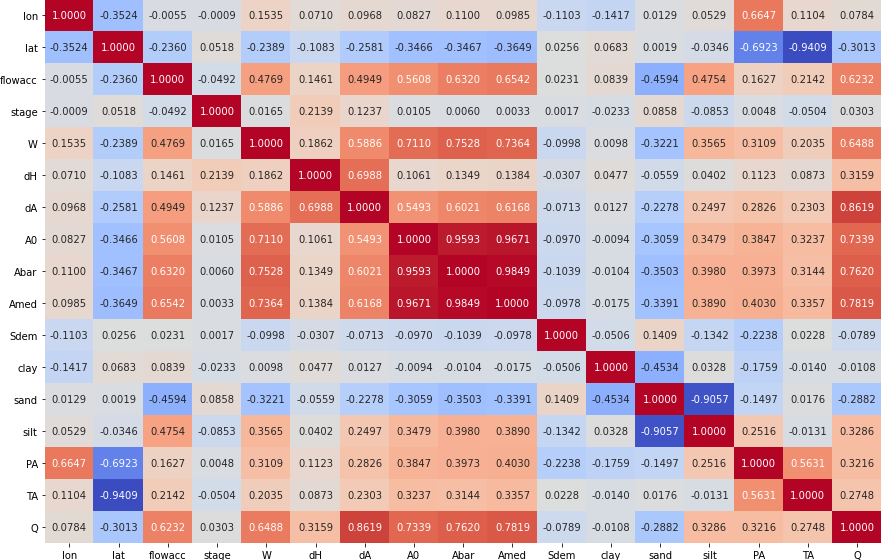
\includegraphics[scale=0.4]{Graph/correlation_hydro.png}
\caption{Correlation matrix of the HydroSwot dataset}
\label{fig:corH}
\end{figure}

For HydroSwot, we see in Figure \ref{fig:corH} that the highest coefficients of correlation with $Q$ are $dA$, $Abar$, $A0$, $Amed$, $W$, and $flowacc$. On the one hand, it makes sense to see $Abar$, $A0$, and $Amed$ so high because they are part of the equation to compute $Q$. On the other hand, $dA$, $W$, and $flowacc$ appear to be variables the most correlated with $Q$. In contrast, $Sdem$ is not highly correlated with $Q$.

\begin{figure}[H]
\centering
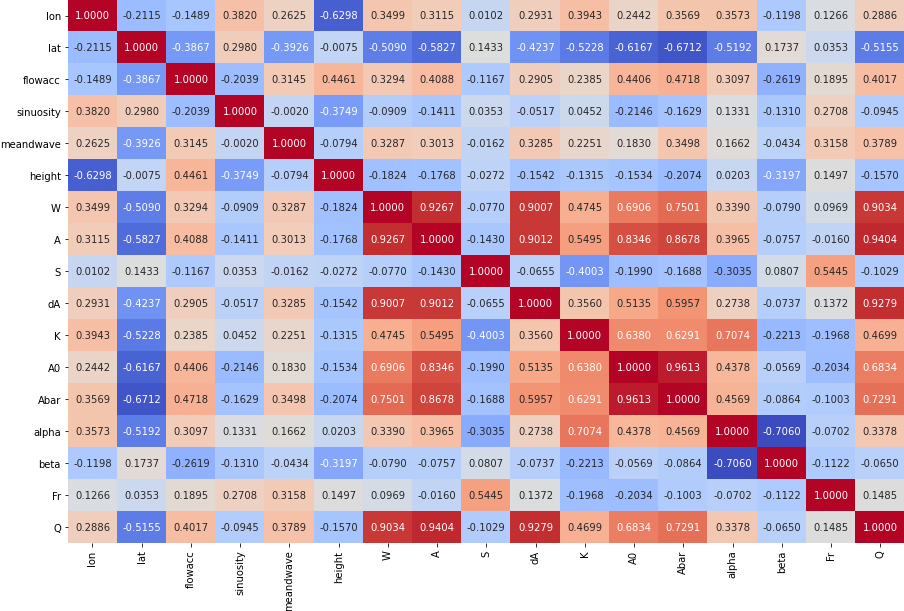
\includegraphics[scale=0.4]{Graph/correlation_pepsi.png}
\caption{Correlation matrix of the PEPSI dataset}
\label{fig:corP}
\end{figure}

For Pepsi, we calculate the correlations in figure \ref{fig:corP}. As for HydroSwot, we observe that $dA$ and $W$ are the two most correlated variables with the river discharge $Q$. But this time, $flowacc$ is much less correlated with $Q$, and the Strickler coefficient $K$ has a high coefficient correlation with $Q$.\newline

To conclude the analysis of the correlation coefficients, the most essential variables that explain $Q$ seem to be $dA$, $W$, and $flowacc$. We verify this conclusion with a Principal Component Analysis. 

\subsubsection{Principal Component Analysis.}

The first step of a PCA is to determine the number of principal components. Due to the high dimension of our datasets, the boxplot of the components is hardly sufficient to determine an optimal number of principal axes (see Figure \ref{fig:pcahydro} and Figure \ref{fig:pcapepsi}). 
 
 \begin{figure}[H]
     \centering
     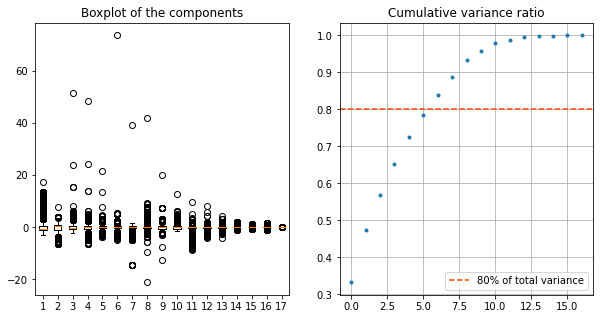
\includegraphics[scale = 0.55]{Graph/hydro_pca.png}
     \caption{Boxplot of the components and cumulative variance ratio plot, HydroSwot dataset}
     \label{fig:pcahydro}
 \end{figure}
 
Although we cannot determine the exact number of components using the boxplot, the plot of the cumulative variance ratio (see Figure \ref{fig:pcahydro}) shows that 6 components are sufficient to almost reach $80\%$ of the total variance for the HydroSwot dataset.

 \begin{figure}[H]
     \centering
     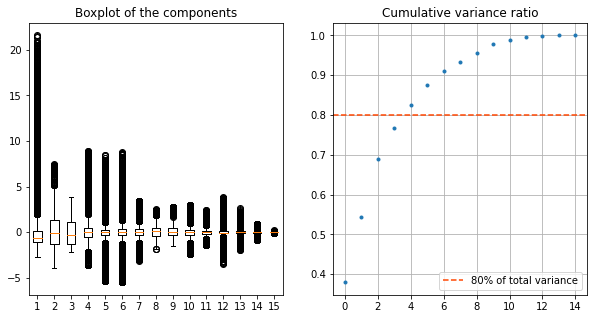
\includegraphics[scale = 0.55]{Graph/pepsi_pca.png}
     \caption{Boxplot of the components and cumulative variance ratio plot, PEPSI dataset}
     \label{fig:pcapepsi}
 \end{figure}

For the PEPSI dataset, 4 components seem to be sufficient. Taking a fifth principal component to reach $80\%$ of the total variance just represents a small ratio of variance, so we decide to take 4 principal axes.

Then, we show the loading plots. We want to find the major interactions, so we focus on the spans formed by the two first principal components (See Figure \ref{fig:factormap}).

\begin{figure}[H]
    \centering
    \begin{subfigure}{0.45\textwidth}
        \centering
        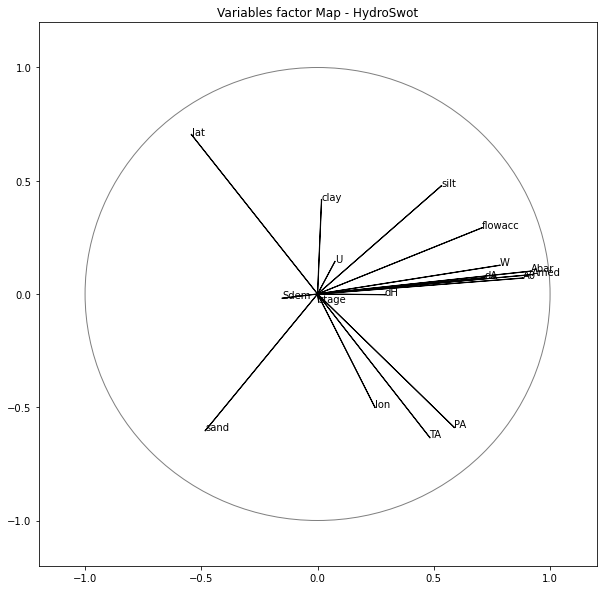
\includegraphics[scale=0.28]{Graph/factor_map_hydro.png}
        \caption{HydroSwot}
        \label{subfig:fmh}
    \end{subfigure}
    \begin{subfigure}{0.45\textwidth}
        \centering
        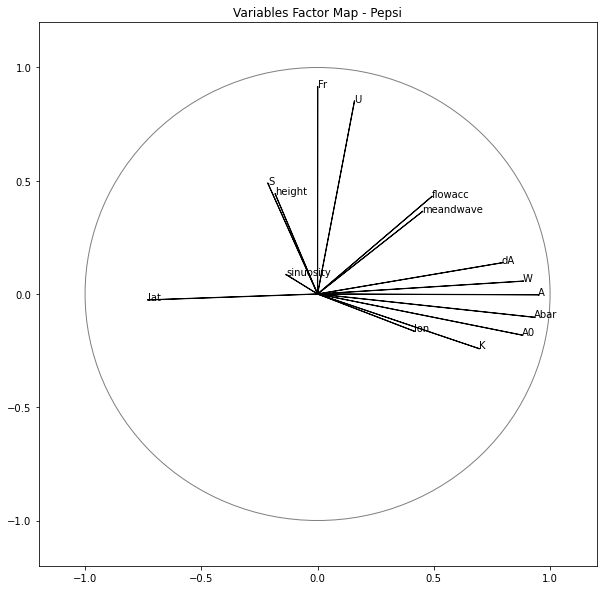
\includegraphics[scale=0.28]{Graph/factor_map_pepsi.png}
        \caption{PEPSI}
        \label{subfig:fmp}
    \end{subfigure}
\caption{Loading plots in the span formed by components 1 and 2}
\label{fig:factormap}
\end{figure}

As we can see on Figure \ref{subfig:fmh}, for HydroSwot, the variables that most explain the principal component are $dA$, $W$, and $flowacc$, as the first two ones are almost parallel to the first axe. We also notice the importance of the composition of the river with $sand$ and $silt$, the meteorological data with $PA$ and $TA$, and finally the geographical position. 

As for HydroSwot, $dA$, $W$, and $flowacc$ are good descriptors of the first component of the PEPSI dataset (see Figure \ref{subfig:fmp}). This time, we observe that the slope $S$ is part of the significant variables. Once again, we observe the importance of the physical metric such as the Froude Number, $Fr$, and the Strickler coefficient, $K$.\newline

Finally, we display the score plots in the span formed by the two principal components (see Figure \ref{fig:scoreplot}).

\begin{figure}[H]
    \centering
    \begin{subfigure}{0.45\textwidth}
        \centering
        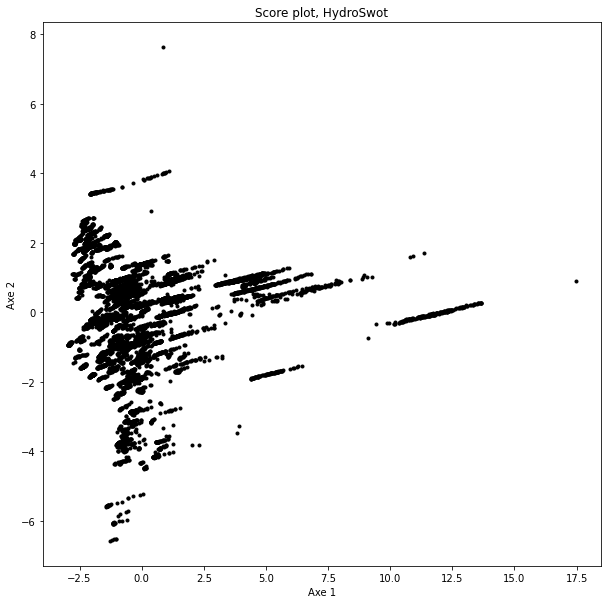
\includegraphics[scale=0.28]{Graph/scoreplot_hydro.png}
        \caption{HydroSwot}
        \label{subfig:sph}
    \end{subfigure}
    \begin{subfigure}{0.45\textwidth}
        \centering
        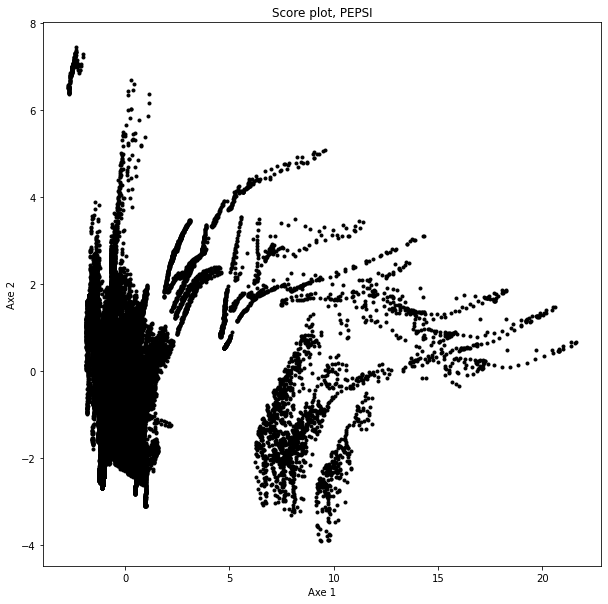
\includegraphics[scale=0.28]{Graph/scoreplot_pepsi.png}
        \caption{PEPSI}
        \label{subfig:spp}
    \end{subfigure}
\caption{Score plots in the span formed by components 1 and 2}
\label{fig:scoreplot}
\end{figure}

Concerning the HydroSwot dataset, we observe in Figure \ref{subfig:sph} that the individuals form lines whose directions are similar to the directions of $dA$, $W$, and $flowacc$ on the loading plot of HydroSwot (see Figure \ref{subfig:fmh}). It stresses the fact that these variables are very significant (see \nameref{section231} section) in this dataset, and it suggests that each line represents all the observations of a particular river.

We see in Figure \ref{subfig:spp} that the individuals from the PEPSI dataset have a singular representation, but it is difficult to analyse the meaning of it. Even so, we notice two different groups, that may correspond to two different scale of river discharge.\newline

To  summarise, the multidimensional analysis leads us to use four input variables for the neural networks : $W$, $dA$, $flowacc$, and the slope ($Sdem$ for HydroSwot, and $S$ for Pepsi, which seems to be more significant than $Sdem$).

\subsubsection{River Classification.\label{section233}} 

To have the most accurate flow estimation, we split rivers into groups. We need to define the number of groups and how to determine them.

We compute a K-means classification for the two datasets with 2 and 3 groups. More groups would lead to too small groups, i.e. with not enough observations to run neural networks algorithms. For both datasets, the K-means classification on 2 groups determines a huge group with the majority of the observations and the other with the rest of the observations. The K-means classification with 3 groups leads to 2 equivalent groups in size and the third group remains small.  

Figure \ref{fig:kmeans} shows a representation of classes by K-means for the HydroSwot dataset. We notice that K-means separates groups distinctly. It also suggests that observations from the same river can be in several groups. K-means classification does not separate rivers between them, it suggests to separate data by river portions.

\begin{figure}[H]
    \begin{subfigure}{0.45 \textwidth}
        \centering
        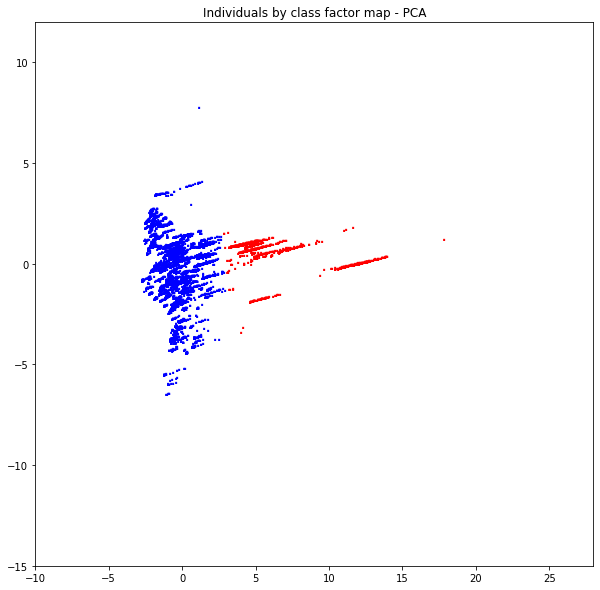
\includegraphics[scale = 0.3]{Graph/kmeans2HS.png}
        \caption{2 classes}
    \end{subfigure}
\centering
    \begin{subfigure} {0.45 \textwidth}
        \centering
        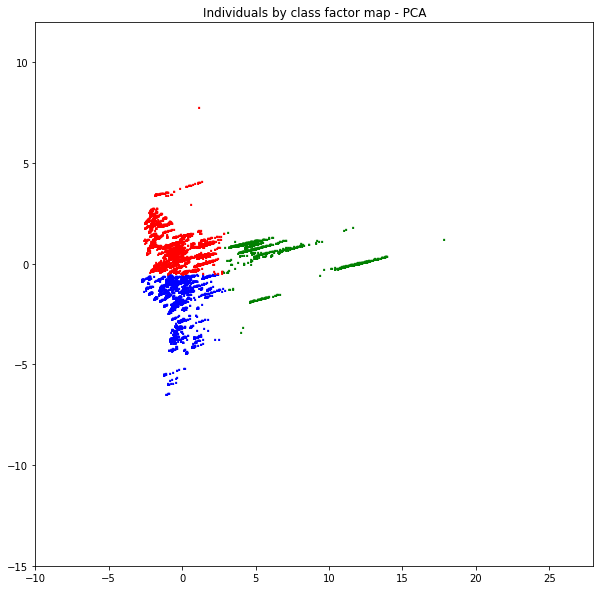
\includegraphics[scale = 0.3]{Graph/kmeans3HS.png}
        \caption{3 classes}
    \end{subfigure}
\caption{Plots for different numbers of classes in the span of the 2 first ACP components for Hydroswot }
\label{fig:kmeans}
\end{figure}

Splitting into 3 groups is not needed for our study. Indeed, we aim to have the largest dataset possible. 

We examine in figure \ref{fig:boxplot_hydro} boxplots of the different variables depending on groups determined by K-means for both datasets. We note that variables which distinct the 2 groups are mainly $Q$ and $flowacc$. $dA$ is also a good separator. \newline

\begin{figure}[H]
\begin{subfigure}{0.45\textwidth }
     \centering
        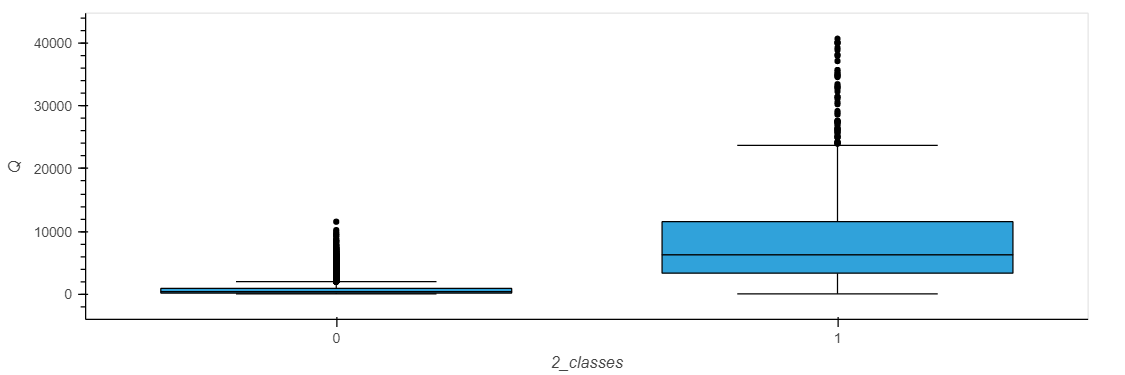
\includegraphics[scale = 0.19]{Graph/bokeh_plot.png}
        \caption{Boxplot of Q}
\end{subfigure}
\begin{subfigure}{0.45\textwidth}
     \centering
        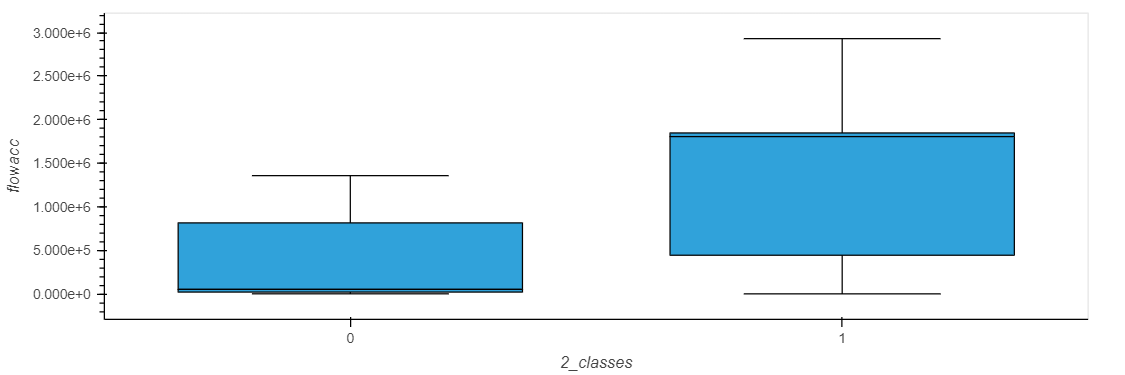
\includegraphics[scale = 0.19]{Graph/flowacc_hydro.png}
        \caption{Boxplot of flowacc }
\end{subfigure}
  \caption{Boxplots of different variables for 2 HydroSwot classes}     
  \label{fig:boxplot_hydro}
\end{figure}

\underline{Remark:} we do not show results of K-means classification for the PEPSI dataset because we obtain the same results and conclusions. \\
    
We finally choose two ways to separate rivers for both datasets. Each method separate rivers into 2 groups as we do not have enough data to create 3 groups.

First, we group data by rivers and compute the river flow mean. We separate them using the criteria of $Q$ which is a good separator according to K-means method. For HydroSwot, we make 2 groups: high discharge rivers ($Q > 1000 m^3/s$) and low discharge rivers ($Q < 1000 m^3/s$). For Pepsi we fix the boundary at $3000 m^3/s$. We notice that the high discharge rivers group for PEPSI contains only 3 rivers: $Mississipi$, $Padma$ and $Jamuna$. This separation by entire rivers is close to the real context of the SWOT Mission. For LSTM network, we will train and test on entire rivers that we know exactly. Then, we will use this algorithm on unknown rivers that the satellite would have measured. We name these separations Hydroswot/PEPSI Handmade - Low/High $Q$.\\

\underline{Remark :} we could separate the datasets using $flowacc$ as we saw that it is also a good separator. \\
The second way to separate data is by following K-means method to split Hydroswot and Pepsi into 2 classes. Among separative variables we have $Q$, so we decide to name the two classes with Low $Q$ and High $Q$. Thus, we obtain Table \ref{Tab:class_prop}.

\begin{table}[H]
\centering
    \begin{tabular}{|c|c|c|}
    \hline
    & Low $Q$ & High $Q$ \\ \hline
    Hydroswot Handmade & 6714 & 5129 \\\hline
    Pepsi Handmade & 47548 & 3721 \\\hline
    Hydroswot K-means  &  10490 & 1140 \\\hline
    Pepsi K-means & 47536 & 2674\\ \hline
    \end{tabular}
\caption{Number of observations in the different classes}
\label{Tab:class_prop}
\end{table}

We notice that HydroSwot K-means - High $Q$ has only 1140 observations. This small number may impact the efficiency of neural networks.

\section{Neural networks setup}

\subsection{Artificial Neural Networks theory. \label{nn}}

The prior methods and materials described are essential to use Artificial Neural Networks (ANN) (Charu C. Aggarwal, 2018 \cite{livre_NN}, M. Albert, P. Besse, B. Laurent, 2020 \cite{cours_ML}). An Artificial Neural Network is non linear with respect to its parameters, noted as $\theta$, that associates to an entry $x$ an output $y = f (x, \theta)$. In this study, our output is uni-dimensional but it can be multidimensional in other applications.\newline

An artificial neuron, inspired by a biological neuron, is composed of : 
\begin{itemize}
    \item[\textbullet] a function $f_j$ of the input $x = \{x_1 \mbox{, ... , }x_d\}$
    \item[\textbullet] a vector of connection weights $w_j = \{w_{j,1} \mbox{, ... , } w_{j,d}\}$
    \item[\textbullet] a neuron bias noted $b_j$
    \item[\textbullet] an activation function $\phi_j$
\end{itemize}

This gives us : 
\begin{equation}
    y_j = f_j(x) = \phi ( <w_j , x> + b_j )
\end{equation}
Figure \ref{fig:neuron} represents an artificial neuron, where $\Sigma$ corresponds to $<w_j,x> + b_j$. 

\begin{figure}[H]
    \centering
    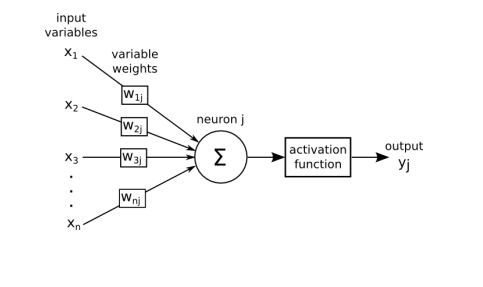
\includegraphics[scale = 1.1]{Graph/neuron.png}
    \caption{Schematic representation of an artificial neuron \cite{cours_ML}}
    \label{fig:neuron}
\end{figure}

A neural network, represented in Figure \ref{fig:neural_network}, is an association of several neurons, grouped in layers, called hidden layers. In this structure, also known as a multi-layer perceptron, the output of each neuron of a layer becomes the input of the neurons of the next layer. A potential different activation function than the hidden layers may be applied on the output layer depending on the problem, classification or regression. After having defined the architecture, we have to estimate the parameters, $w_j$ (grouped in matrix $W$) and $b_j$ (grouped in vector $b$), with a training sample and the back propagation algorithm. 

\begin{figure}[H]
    \centering
    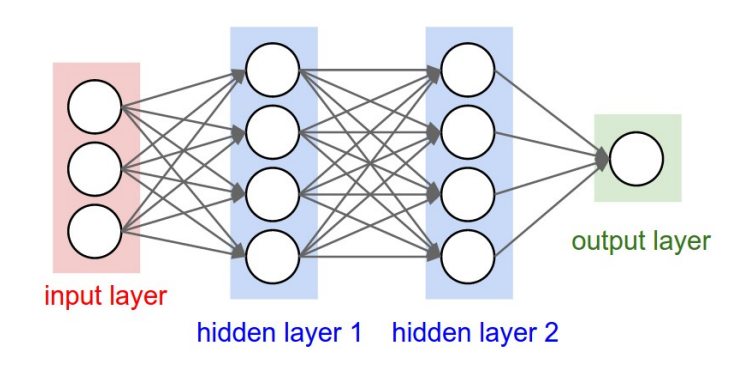
\includegraphics[scale = 0.7]{Graph/neural_net.png}
    \caption{Schematic representation of the architecture of a neural network \cite{cours_ML}}
    \label{fig:neural_network}
\end{figure}
A neural network is executed as follows : 
\begin{itemize}
    \item We select the explanatory variables used to train the network. The input data needs to be scaled whereas the output - the discharge in our case - does not need to be scaled. Then we split our dataset into a training set and a testing set, with a proportion of $80-20\%$.
    \item We choose a loss function. The main loss functions that we will use are Mean Absolute Error ($MAE$) and Mean Square Error ($MSE$). (See section \nameref{metrics})
    \item We randomly initialize the parameters $W$ and $b$. 
    \item We set $h^{(0)}(x) = x$. We compute at each hidden layer $k$, $h^{(k)}(x) = \phi (Wh^{(k-1)}(x)+b^{(k)})$ where $x$ is the input data. Then we compute the predicted values. This is the \textit{forward} phase. 
    \item We minimize a loss function, generally with a gradient descent algorithm, to find optimal $W$ and $b$. The gradient is computed with the backpropagation algorithm and the backpropagation equations. This is computed on subsets, called batches,  to optimize the computation time. Then, the values obtained are used to update the parameters $W$ and $b$. This is the \textit{backward} phase. 
    \item We iterate the \textit{forward} and the \textit{backward} phases a number of times called $epochs$ that we define.\newline
\end{itemize}

Le Cun (1986) \cite{lecun1989backpropagation} proposed the backpropagation algorithm which is an efficient way to compute the gradient of a neural network. It allows to easily obtain a local minimizer of the quadratic criterion. The idea is to recursively compute the gradient through the hidden layers. 

The success of the neural networks came from an universal approximation theorem due to Hornik (1991) \cite{hornik1991approximation}. This theorem shows that any bounded function can be approximated by a network with a single hidden layer, a finite number of neurons and a single activation function. 


\subsection{Long Short-Term Memory Networks.}

Long Short-Term Memory (LSTM) has been introduced by Sepp Hochreiter and Jürgen Schmidhuber in 1997 \cite{lstm_createur}. A LSTM is a Recurrent Neural Network (RNN). The main quality of a RNN and so of a LSTM network is that they can manage the time dependence contrary to classical neural networks.

To compute a RNN, we have to choose the number of memory layers, $K$. If $K$ is too big, the number of parameters increases too much. It becomes too complicated to learn the weights due to the vanishing gradient. RNN does not have a long term memory. In our case we need a long term memory. We must use LSTM networks.\newline

A LSTM includes an input gate, an output gate and a forget gate. A LSTM has its own memory $c$. Figure \ref{fig:lstm cell} shows the architecture at time $t$ of a LSTM cell.

\begin{figure}[H]
    \centering
    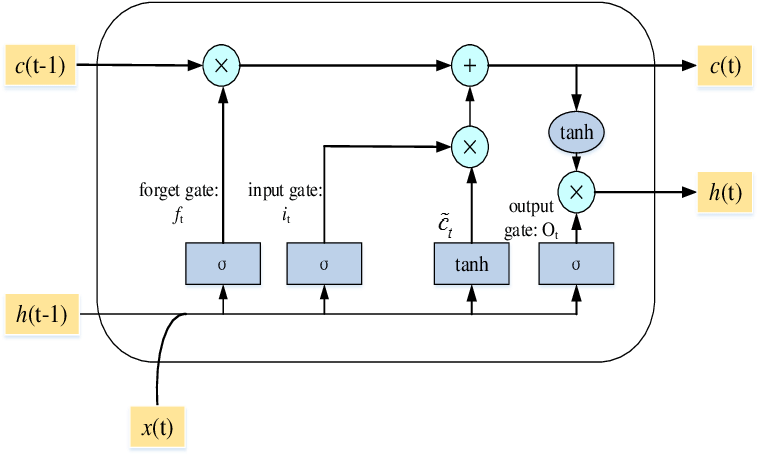
\includegraphics[scale = 0.4]{Graph/cellule_lstm.png}
    \caption{Schematic representation of a LSTM cell \cite{lstm_cell}}
    \label{fig:lstm cell}
\end{figure}

It works as follows :
\begin{itemize}
    \item The forget gate is used to "forget" useless information. $f_t = \sigma(W, [h(t-1), x(t)] + b_f)$
    \item The input gate proposes new information to put into the cell memory. $\tilde{C}_t = tanh(W, [h(t-1), x(t)] + b_f)$ corresponds to what information we put into the cell memory. $i_t = \sigma(W, [h(t-1), x(t)] + b_f)$ corresponds to the quantity of information we add.
    \item We use the two previous gates to compute the cell memory : $c(t) = c(t-1) f_t + i_t \tilde{C}_t $
    \item The output gate : $O(t) = \sigma(W, [h(t-1), x(t)] + b_f)$.
    \item Finally, $h(t) = O(t) + tanh(c(t))$ is calculated. It defines the output of the cell using the cell memory $c(t)$ and $tanh$ which determines what information to take from the memory.
\end{itemize}

Moreover, $\sigma$ is the sigmoid function, and $\{..., x_{t-1}, x_t, x_{t+1}, ... \}$ is the input time series.\newline

LSTM are linked in the way showed in figure \ref{fig:schema lstm}. In this illustration, we have 3 LSTM cells. 

\begin{figure}[H]
    \centering
    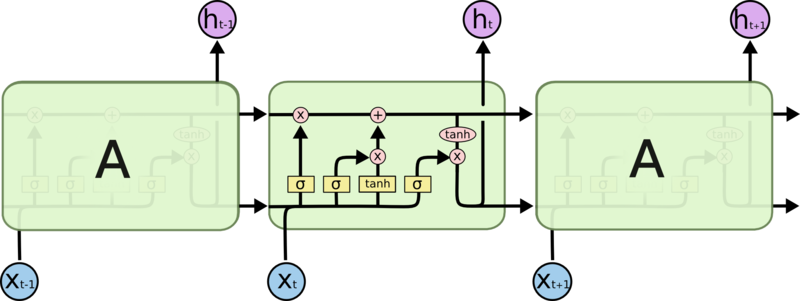
\includegraphics{Graph/schema_lstm.png}
    \caption{Schematic representation of the architecture of a LSTM network \cite{lstm-cell-linked}}
    \label{fig:schema lstm}
\end{figure}

To optimize the weight and the bias of each cell, we use the backpropagation of the gradient (detailed in previous section \nameref{nn}).

\subsection{Performance criteria. \label{metrics}} To evaluate the performances of a neural network, we quantify the errors using different criteria called metrics. 

\subsubsection{Useful common metrics.\label{section321}}
 We compute the \textit{Mean Square Error}, denoted by $MSE$, and defined in (\ref{eq:mse}).
\begin{equation}
    MSE(y) = {\frac{1}{n} \left( \sum^n_{i=1}(y^{est}_i - y^{obs}_i)^2 \right)}
    \label{eq:mse}
\end{equation}
with $y^{est}_i$ the $i^{th}$ estimation and $y^{obs}_i$ the true value associated.\\

\textit{Mean Absolute Error}, denoted by $MAE$ has a physical meaning, as it does not modify the values of the river discharge. Using the same notations as previous, $MAE$ is defined in (\ref{eq:mae}).
\begin{equation}
    MAE(y) = {\frac{1}{n} \left( \sum^n_{i=1}\lvert y^{est}_i - y^{obs}_i\rvert \right)}
    \label{eq:mae}
\end{equation}

 The \textit{Pearson correlation coefficient}, denoted by $R2$ is set in (\ref{eq:r2}).
\begin{equation}
    R2(y) = \frac{\sum_{i=1}^{n}(y^{est}_i - \bar y^{est}) (y^{obs}_i - \bar y^{obs})} {\left(\sum_{i=1}^{n}(y^{est}_i - \bar y^{est})^2\right)^{1/2}\left(\sum_{i=1}^{n}(y^{obs}_i - \bar y^{obs})^2\right)^{1/2}}
    \label{eq:r2}
\end{equation}

where $\bar y^{est}$ the average value of the estimations and $\bar y^{obs}$ the average value of the validation values.\newline

We define the \textit{Root Mean Square Error} in (\ref{eq:rmse}), denoted by $RMSE$ and the \textit{Normalized Root Mean Square Error}, denoted by $nRMSE$ in (\ref{eq:nrmse}).
\begin{equation}
    RMSE(y) = \sqrt {\frac{1}{n} \left( \sum^n_{i=1}(y^{est}_i - y^{obs}_i)^2 \right)}
    \label{eq:rmse}
\end{equation}

\begin{equation}
    nRMSE(y) = \frac{RMSE(y)} {\bar y^{obs}}
    \label{eq:nrmse}
\end{equation}

% \subsubsection{Useful metrics in hydrology.}

% Then, we define two other metrics specific to hydrology. The first one is the \textit{Nash-Sutcliffe model Efficiency}, denoted by $NSE$ and defined in (\ref{eq:nse}) with the same notations defined in \nameref{section321} section. The second one is the \textit{Kling-Gupta model Efficiency}, denoted by $KGE$ in (\ref{eq:kge}).
% \begin{equation}
%     NSE(y) = 1 - \frac{\sum^n_{i=1}(y^{est}_i - y^{obs}_i)^2} {\sum^n_{i=1}(y^{obs}_i - \bar y^{obs})^2}
%     \label{eq:nse}
% \end{equation}

% \begin{equation}
%     KGE(y) = 1 - \sqrt {(\beta_{KG}-1)^2+(\alpha_{KG}-1)^2+(R^2-1)^2}
%     \label{eq:kge}
% \end{equation}
% where $\beta_{KG}=\frac{\bar y^{est}}{\bar y^{obs}}$ and $\alpha_{KG} = \frac{\sigma(y^{est})}{\sigma(y^{obs})}$.

\subsubsection{Physical criteria : Low-Froude model.}

The last criteria we define is the Low-Froude model. The objective is to match physical criteria with a neural network. In our case, we want to know if the predicted river flow follows the Low-Froude model. The Strickler friction coefficient $K$ can be defined as a local power law (K. Larnier, J.Monnier, 2020 \cite{larnier2020hybrid}), i.e. for a given reach $r$ and an instant $p$, as shown in (\ref{eq:MS_law}): 

\begin{equation}
    K_{r,p} = \alpha_r \left( Z_{r,p} - Z{r,0} + \frac{1}{W-{r,0}}A_{0,r}\right)
    \label{eq:MS_law}
\end{equation}

where $\alpha$ and $\beta$ are Manning-Strickler coefficients.\newline

Using the Manning-Strickler law and (\ref{eq:MS_law}), (\ref{eq:low froude}) defines the algebraic Low-Froude flow model, a system of $R$ equations, where $R$ is the number of reaches : 
\begin{equation}
    Q^{3/5}_{r,p} = \alpha_r^{3/5} ( c_{r,p}^{(1)} A_{0,r} + c_{r,p}^{(2)})(c_{r,p}^{(4)}A_{0,r} + c_{r,p}^{(3)})^{3/5\beta_r}
    \label{eq:low froude}
\end{equation}
with : $ c_{r,p}^{(1)} = W_{r,p}^{-2/5}S_{r,p}^{3/10}$, $ c_{r,p}^{(2)} = c_{r,p}^{(1)} \partial A_{r,p}$, $ c_{r,p}^{(3)} = (H_{r,p} - H_{r,0})$, and  $ c_{r,p}^{(4)} = \frac{1}{W_{r,0}}$. These coefficients can be computed with altimetry measurements. 
\section{Numerical analysis and discussion}
\subsection{Artificial Neural Networks results}

\subsubsection{Data preparation.\label{section411}}

As explained in the previous section (see \nameref{section233} section), we separate our datasets into classes. These classes are defined by K-means or by hand. We also have a difference in the training/testing splitting phase, where we can split the data considering all the observations, or just by considering full rivers. Hence, we compute several neural networks on the following subsets.

\begin{table}[H]
    \centering
    \begin{adjustbox}{max width=\textwidth}
    \begin{tabular}{|c|c|c|c|c|c|}
    \hline
        Dataset & Class. method & Class & Split. method & Name of the subset & abbreviation\\ \hline \hline
        HydroSwot & Handmade & Low $Q$ & Observations & HydroSwot Handmade - Low Q & h\_LQ\\ \hline
        HydroSwot & Handmade & High $Q$ & Observations & HydroSwot Handmade - High Q &h\_HQ\\ \hline
        HydroSwot & Handmade & Low $Q$ & Full rivers & HydroSwot Handmade Full rivers - Low Q &h\_LQ\_R\\ \hline
        HydroSwot & Handmade & High $Q$ & Full rivers & HydroSwot Handmade Full rivers - High Q& h\_HQ\_R\\ \hline
        HydroSwot & K-means & Low $Q$ & Observations & HydroSwot K-means - Low Q &h\_K\_LQ\\ \hline
        HydroSwot & K-means & How $Q$ & Observations & HydroSwot K-means - How Q &h\_K\_HQ\\ \hline
        PEPSI & Handmade & Low $Q$ & Observations & PEPSI Handmade - Low Q& p\_LQ\\ \hline
        PEPSI & Handmade & High $Q$ & Observations & PEPSI Handmade - High Q& p\_HQ\\ \hline
        PEPSI & Handmade & Low $Q$ & Full rivers & PEPSI Handmade Full rivers - Low Q&p\_LQ\_R\\ \hline
        PEPSI & Handmade & High $Q$ & Full rivers & PEPSI Handmade Full rivers - High Q&p\_HQ\_R\\ \hline
        PEPSI & K-means & Low $Q$ & Observations & PEPSI K-means - Low Q&p\_K\_LQ\\ \hline
        PEPSI & K-means & How $Q$ & Observations & PEPSI K-means - How Q&p\_K\_HQ\\ \hline
    \end{tabular}
    \end{adjustbox}
    \caption{Training subsets of HydroSwot and PEPSI datasets}
    \label{tab:classes}
\end{table}

Each dataset is randomly separated in training and testing sets with an 80\% and 20\% proportion, respectively for the training and the testing sets. We notice that these proportions are not exactly respected for handmade full river datasets. This is due to the constraint of extracting full rivers from the initial dataset. 

In section \nameref{variables_selection}, we determined the features to use in the neural networks. Hence, we use $W$, $dA$, $flowacc$, and the slope ($Sdem$ for HydroSwot, and $S$ for Pepsi). 

\subsubsection{Architecture of the neural networks.}

Before training neural networks, we must decide of its architectures. First, we need to determine the number of layers and the number of neurons in each layer. These parameters depend on the shape of the data we will train the ANN with, so the architecture is different depending on the dataset. 

A large dataset such as PEPSI Handmade - Low Q requires an ANN with more layers and neurons than a dataset like HydroSwot K-means - High Q. To determine the best architecture, we build several neural networks for each dataset, and compare their efficiency through different metrics: \textit{Mean Squared Error} and \textit{Mean Absolute Error}.

As a result, we choose for PEPSI - Low Q datasets a neural network with 32 layers containing 32 neurons. We choose 8 layers and 8 neurons in each PEPSI - High Q datasets. For HydroSwot datasets, we choose 16x16 neural network depending for all the subsets, except the K-means - High Q one, which has a 8x8 architecture. We aim to have more data in the training set than the number of parameters in the neural network.

Regarding the parameters of the ANN, 100 epochs are enough for the algorithm to converge. We choose a batch size of 25. We use the \textit{Mean Square Error} (MSE) as loss function. 

\subsubsection{Artificial Neural Network training.}

To estimate the goodness of fit of the neural network, we use the two different metrics, $MAE$ and $MSE$. We plot the results. We aim to observe a convergence.  Each graph in Figure \ref{fig:subploth} represents one of the 6 HydroSwot classes presented in Table \ref{tab:classes}.

\begin{figure}[H]
    \centering
    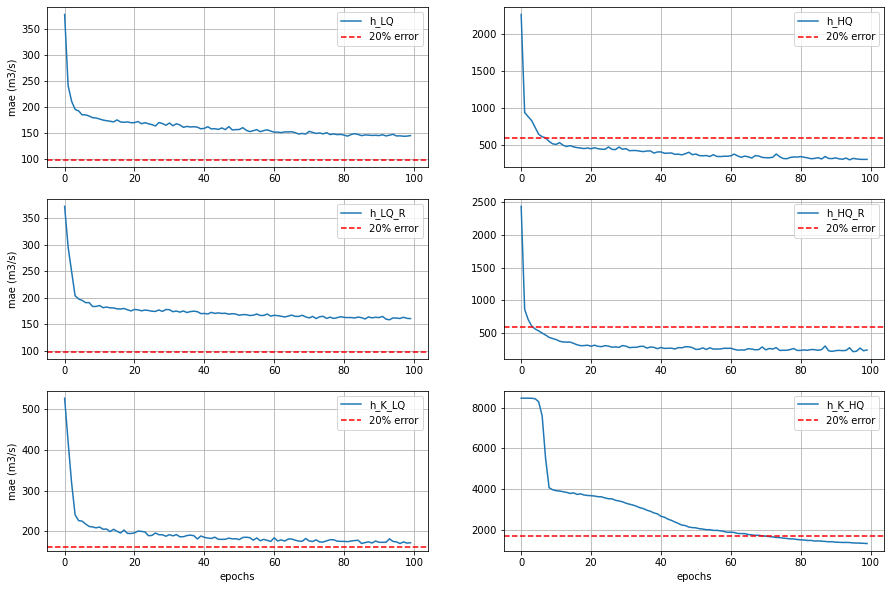
\includegraphics[scale = 0.45]{Graph/subplot_mae_h.png}
    \caption{Goodness of fit of the neural network for each HydroSwot class}
    \label{fig:subploth}
\end{figure}

We see that all the curves decrease suddenly during the first epochs, then much more slowly, and that they finally converge. We observe that the $MAE$ of the High Q classes always decreases below the 20\% error rate, while the $MAE$ of the Low Q classes does not.

Specifically, in the cases where the $20\%$ error limit is reached, the goodness of fit of the neural networks is very satisfying. However, having a goodness of fit as precise can lead to over fitting. We can explain this accuracy by the low number of data in each classes (see table \ref{Tab:class_prop}).

Concerning the curves which never reach the 20\% error limit, the goodness of fit of the neural networks is not as accurate as excepted. The fitting is difficult because of the high number of data and the variety of measurements in both classes.

Finally, the $MAE$ curve for the Hydroswot K-means - Low Q class decreases suddenly and stays just above the 20\% error rate, which is more accurate that the two other Low Q classes. In this case, the goodness of fit of the neural network is almost as precise as expected.

\begin{figure}[H]
    \centering
    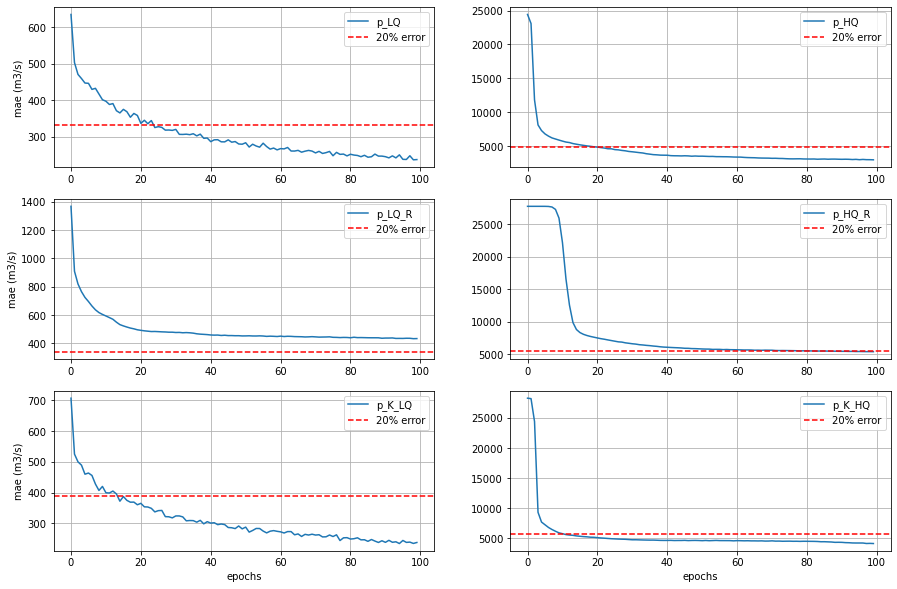
\includegraphics[scale = 0.45] {Graph/mae_subplot_pepsi.png}
    \caption{Goodness of fit of the neural network for each PEPSI class}
    \label{fig:mae pepsi}
\end{figure}

Figure \ref{fig:mae pepsi} shows the $MAE$ through the epochs for all the PEPSI classes. 
The $MAE$ behaviour for high Q classes is similar between them. The curves go closely under the 20\% of error rate. So, the goodness of fit is as expected. For the PEPSI handmade low Q full rivers class, the curve converges above the 20\% of error. Finally, the other low Q classes converge around 15\%. A hypothesis of this rate is the low number of rivers in these classes.   

\subsubsection{Artificial Neural Network testing.}

After the training of our neural networks, we evaluate their performances. Thus, we use the testing set - not used during the learning - to predict river discharge. First, we focus on the HydroSwot classes results. We verify the robustness of our neural networks with a Monte-Carlo method. Indeed, depending of the initialization of training and testing sets we obtain different results.  We initialize 20 times the training and testing sets, always with the same parameters. Then, we run the learning phase. We hence obtain results for 20 neural networks per classes. To quantify precisely the robustness of neural networks, we calculate the \textit{Normalized Root Mean Square Error} for all our classes. In Figure \ref{fig:MontecarloHydro}, we display the boxplots of the errors for all the HydroSwot classes.

\begin{figure}[H]
    \centering
    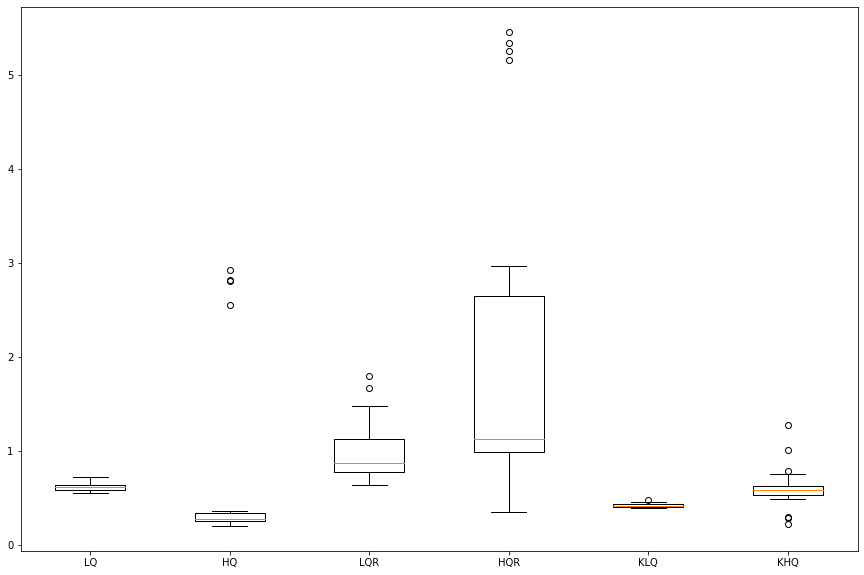
\includegraphics[scale = 0.3]{Graph/MonteCarlo_hydro.png}
    \caption{Boxplots of the \textit{nRMSE} errors for all HydroSwot classes}
    \label{fig:MontecarloHydro}
\end{figure}

 We clearly observe that the classes where we have full rivers contain much more errors, as the medians of the two boxplots are close to 1, and their ranges are much larger than the ones of other classes. Concerning the remaining boxplots, we show that the one with the best median is the HydroSwot Handmade - High Q, while the one with the smallest range is the HydroSwot K-means - Low Q. We also observe that high Q classes contains outliers, as opposed to the low Q classes, which are more robusts.

As a conclusion, classes which do not take full rivers present much better results. We also notice that the high Q classes can obtain the best predictions, but with a higher variance.


Now, we focus on PEPSI results. We plot the predictions (on the horizontal axis) against the real values (on the vertical axis). In figure \ref{fig:predictionsANN}, our predictions are computed on the PEPSI K-means classes.

\begin{figure}[H]
    \begin{subfigure}{0.45 \textwidth}
        \centering
        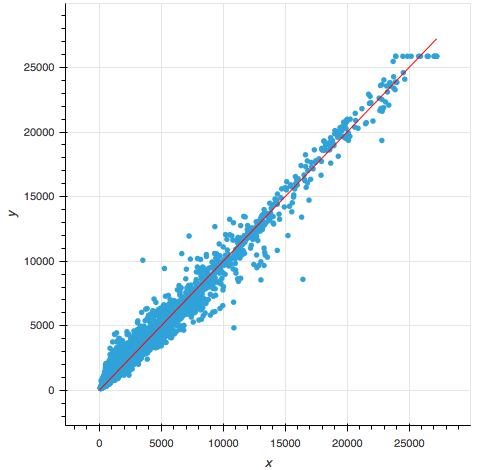
\includegraphics[scale = 0.4]{Graph/predictions_pepsiK_LQ.png}
        \caption{Low river discharge}
        \label{subfig:predLQ}
    \end{subfigure}
    \centering
     \begin{subfigure}{0.45 \textwidth}
         \centering
        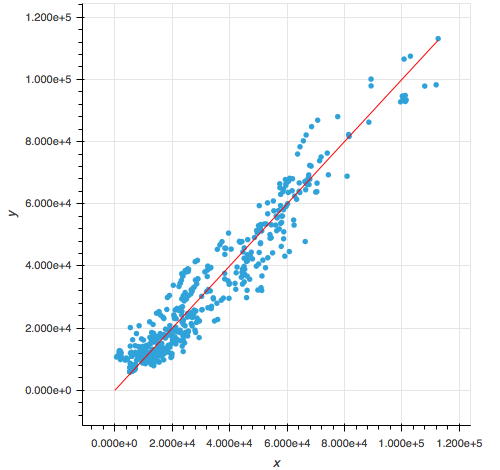
\includegraphics[scale = 0.4]{Graph/predictions_pepsiK_HQ.png}
        \caption{High river discharge}
        \label{subfig:predHQ}
     \end{subfigure}
 
 \caption{Predictions against real values of the neural network, PEPSI K-means - Low Q and High Q}
 \label{fig:predictionsANN}
\end{figure}

Figure \ref{subfig:predLQ} represents the predictions for low river discharges. We observe that the majority of the predictions are close to the red line, which means that a prediction is close to its real measure. We just observe some outliers, but their number is very small. In Figure \ref{subfig:predHQ}, we represent the predictions for high river discharges. Here, the predictions are further away from the red line. We assume this is due to the much smaller number of observations contained in this class compared to the low Q class. The predictions are good though.

Then, to focus on the predictions of a river in particular, we plot the predicted hydrographs of the rivers of the testing set, and we compare them to their true measures. Noteworthy that the hydrographs are only plotted when we use the classes with full rivers, since the other classes already use some observations of the rivers during training. The hydrographs can also be obtained only on the PEPSI dataset, because it is in this dataset that we have daily observations. Here, the following hydrographs (cf. Figure \ref{fig:hydrographKushiyara}, Figure \ref{fig:hydrographOhio}) come from the PEPSI Handmade Full rivers - Low Q class. 

\begin{figure}[H]
    \centering
    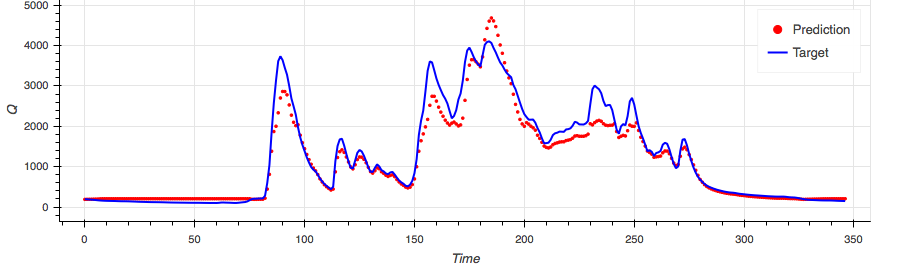
\includegraphics[scale = 0.4]{Graph/Hydrogramme_Kushiyara.png}
    \caption{Hydrograph of river $Kushiyara$, PEPSI low Q full river class}
    \label{fig:hydrographKushiyara}
\end{figure}
\begin{figure}[H]
    \centering
    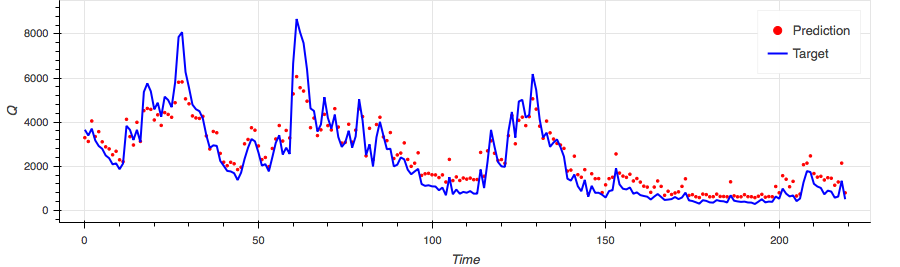
\includegraphics[scale = 0.4]{Graph/Hydrogramme_OhioSection2.png}
    \caption{Hydrograph of river Ohio - section 2, PEPSI low Q full river class}
    \label{fig:hydrographOhio}
\end{figure}

The accuracy of the predicted hydrographs vary depending on the river. We observe that the predicted hydrograph of river $Kushiyara$ fits well the real hydrograph: there is no temporal bias, all the peaks are present, and their values are close to reality (never more than a $800 m^3/s$ difference). However, the predicted hydrograph of river Ohio - Section 2 contains more bias while trying to predict the peaks, but there is again no temporal bias. 


\begin{table}[H]
    \centering
    \begin{tabular}{|c|c|}
    \hline
    Class & nRMSE \\ \hline \hline 
         p\_HQ& 0.19 \\ \hline
         p\_LQ& 0.32\\ \hline
         p\_HQ\_R & 2.46\\ \hline 
         p\_LQ\_R & 0.85\\ \hline
         p\_K\_HQ & 0.19\\ \hline
         p\_K\_LQ & 0.25\\ \hline
    \end{tabular}
    \caption{nRMSE calculated on testing sets for PEPSI classes}
    \label{tab:nRMSE-PEPSI}
\end{table}

Table \ref{tab:nRMSE-PEPSI} resumes neural networks performances for all PEPSI classes on testing set. The PEPSI Handmade Full rivers - High Q class does not have an accurate result. For this class, the training set is composed of 2 rivers and the testing set of only one river. Despite of the convergence of the $MAE$ to the 20\% of error rate (shown in figure \ref{fig:mae pepsi}), the neural network does not permit to estimate accurately the discharge of the third river. The PEPSI Handmade Full rivers - Low Q class does not have satisfying result. The reason can be the low number of river that the class have.


PEPSI Handmade - Low Q  and PEPSI K-means - Low Q classes have a $MAE$ on training set which decreased lower than the PEPSI Handmade - High Q and PEPSI K-means - High Q. However, their $nRMSE$ on testing set are worse than the other 2 classes. Hence, this result illustrates the phenomenon of over-fitting. 

We conclude of a good estimation of the discharge for all the PEPSI classes except for the full rivers ones.   
\subsection{Neural Networks training LSTM}

\subsubsection{Data preparation.}

LSTM neural networks are based on time series. Hence, we can only use the PEPSI dataset where the variable $day$ is present. The measurement sequences available in PEPSI goes from 145 days to a maximum of 595 days depending on the river. LSTM neural networks learn from a single river time series. Therefore, the time series we have are too small. We need to periodise the time series over several years to obtain a sufficiently large dataset and a pattern that repeats over the years. We assume that the river flow rate is the same over the years. Because of this size problem, we focus our study on the \textit{Missouri Downstream} river which has observations for 595 days. We first cut the time series around 360 days to have a full year. We also have to cut it at a day where the river discharge is close to the first day river discharge to have continuity between each year. Once this compromise has been found, we can periodise the time series of \textit{Missouri Downstream} river. 

\begin{figure}[H]
    \begin{subfigure}{0.45 \textwidth}
        \centering
        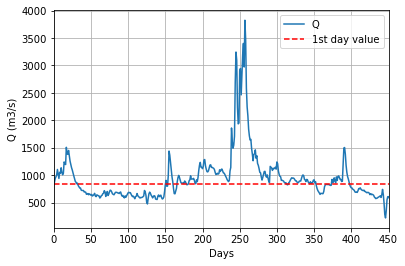
\includegraphics[scale = 0.5]{Graph/1year.png}
        \caption{Initial time series}
        \label{fig:my_label}
    \end{subfigure}
    \centering
     \begin{subfigure}{0.45 \textwidth}
         \centering
        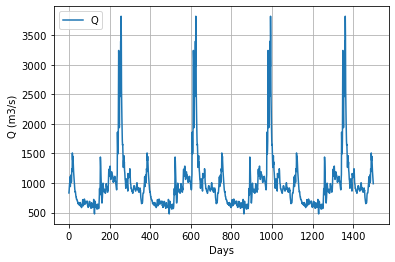
\includegraphics[scale = 0.5]{Graph/5years.png}
        \caption{5 years of river flow after the periodisation}
        \label{fig:periodisation}
     \end{subfigure}

  \caption{Periodisation of \textit{Missouri Downstream} river flow}
  \label{fig:period_Mis}
\end{figure}

 We periodise on $5$ years. Figure \ref{fig:period_Mis} shows the periodisation of the initial time series and then the new river discharge on 5 years.

\subsubsection{Architecture of the neural networks.}

We choose 80\% - 20\% for the proportion between the training and the testing set. We set the sequence length at 16, i.e. the number of days used to predict the next day, and the batch size also to 16. We change the features used for the learning phase. \textit{Flowacc} is now constant in the time series because we consider a single river and a single reach. Thus, we put \textit{W}, \textit{dA} and \textit{S} as input data, and \textit{Q} always as output data. \\

For \textit{Missouri Downstream} river, we obtain a training set composed of 2944 days, and 736 days for the testing set. We hence get 91 batches available for the training. We build a neural network with 10 LSTM cells which give us 571 trainable parameters. Mean Squared Error is set as the loss function and as a metric, and Mean Absolute Error and nRMSE as other metrics. Finally, we run the neural networks trough 20 \textit{epochs}. 

\subsubsection{Long Short-Term Memory Network training.}
We compute and display the metrics MAE and nRMSE through the $epochs$ (see Figure \ref{fig:metricsLSTM}). 
\begin{figure}[H]
    \begin{subfigure}{0.45 \textwidth}
        \centering
        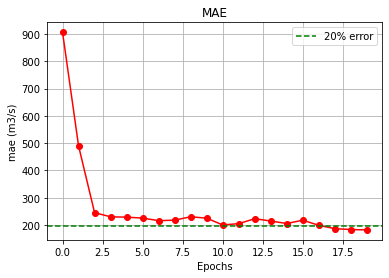
\includegraphics[scale = 0.5]{Graph/mae_lstm.png}
        \label{fig:my_label}
    \end{subfigure}
    \centering
     \begin{subfigure}{0.45 \textwidth}
         \centering
        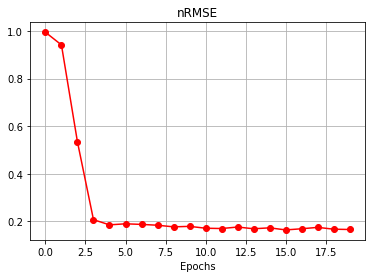
\includegraphics[scale = 0.5]{Graph/nrmse_lstm.png}
        \label{fig:my_label}
     \end{subfigure}
     \caption{Evolution of $MAE$ and $nRMSE$ during the learning phase}
     \label{fig:metricsLSTM}
     
\end{figure}

First, we note the steep and rapid decrease of both of the metrics and the beginning of their convergence from the fifth epoch. MAE converges slowly from the fifth epoch onwards and finally reaches the 20\% physical error rate. The nRMSE also decrease slowly from the fifth epoch under 
20\% of error. Each metrics converge stably to a satisfying rate.  

\subsubsection{Long Short-Term Memory Network testing.}

We compute now the river flow prediction computed on the testing test, and the solution of the Low-Froude model computed with the prediction given by the LSTM network. In table \ref{tab:perf_lstm}, we display the performance of each prediction with nRMSE.

\begin{figure}[H]

\centering
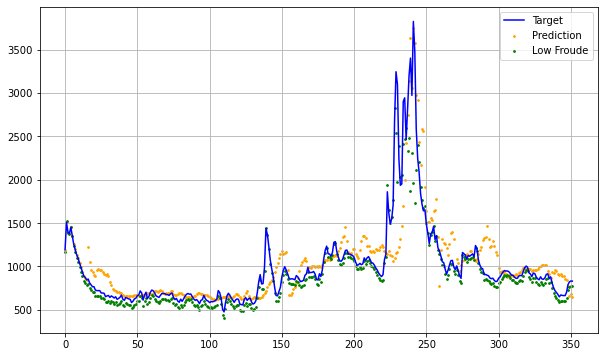
\includegraphics[scale = 0.5]{Graph/pred_low_fr_missour_lstm.png}
\caption{Prediction of $MissouriDownStream$ by LSTM and Low-Froude Model}
\label{fig: lest result} 
\end{figure}

\begin{table}[H]
    \centering
    \begin{tabular}{|c|c|}
    \hline 
        
         Q predicted & 0.28626674 \\
         \hline 
         Low-Froude model & 0.31700262 \\
    \hline
    \end{tabular}
    \caption{nRMSE Performance of the models}
    \label{tab:perf_lstm}
\end{table}

In Figure \ref{fig: lest result}, we observe 3 different hydrographs \textit{Missouri Downstream} river. Each one are close to each other. River discharge seems to be well estimated. The nRMSE of the prediction by LSTM network and the river flow rate computed by the Low-Froude model are around 30\% of error. The results obtained are hence satisfying. Only the prediction of the highest peak of river discharge observed around day 230, what we would expect to be a flood, appears to be less accurate than the smaller peaks. The low nRMSE of the solution of the Low-Froude model shows us that LSTM prediction is consistent with the Low-Froude model. 
We conclude that the architecture of LSTM enables to predict accurately discharge values for this river. The condition to obtain such results is to have enough data, and so to have enough days / years to train on. Hence, we see that a good solution is the duplication of an existing time series as we perform in our study.

\subsection{Discussion.}

As a conclusion, we computed two different neural networks, which have two different aims.

First, the Artificial Neural Network is a versatile neural network, as it can predict the river discharge on any river. But the quality of the prediction will depend nearly exclusively on the amount of data available : to be efficient, the ANN needs to train itself on a huge dataset in terms of size.

Second, the Long Short-Term Memory network is at the opposite of the Artificial Neural Network : it does not need a huge amount of data, as 5 years of data from a river are sufficient, which represents a small dataset size. However, the network can just predict the river discharge of a particular river, which can be restrictive.\newline

Thus, the common and crucial point is the following : to be efficient, the two neural networks need an important amount of data. In this way, the SWOT mission seems to be perfectly adapted, as it will collect many river data around the world.\newline

We will finish by mentioning the following point. During this study, we discriminated our rivers according to their river discharges. But actually, we will not possess this information about the new rivers we will want to predict the river discharge. Thus, separate the rivers according to other criteria, such as the flow accumulation or the width, could be a solution. A more precise discrimination could even be to separate the data according to river reaches, and not just on entire rivers.
\newpage

\bibliographystyle{siamplain}
\bibliography{bibtex}

% % 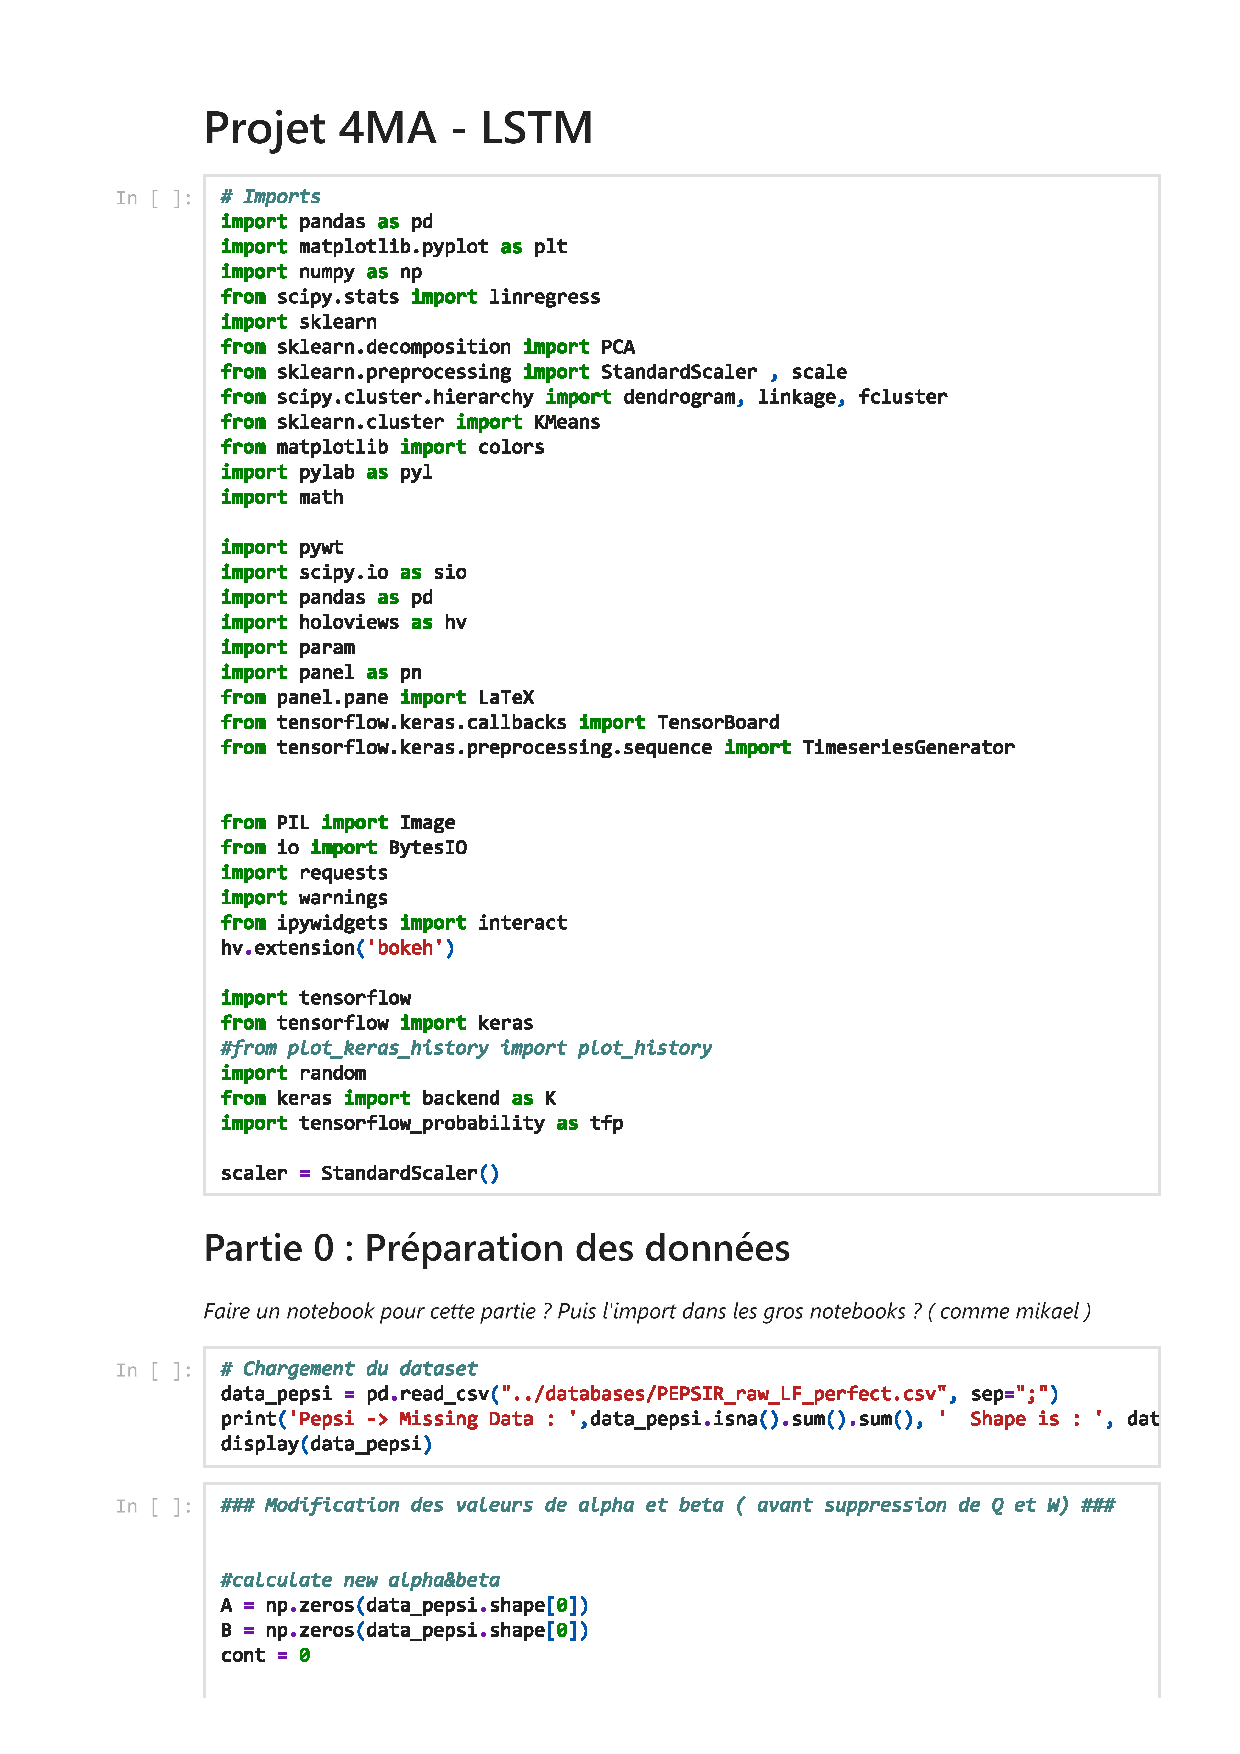
\includepdf[pages=-]{pdf_lstm.pdf}
% \section{Annex}
% 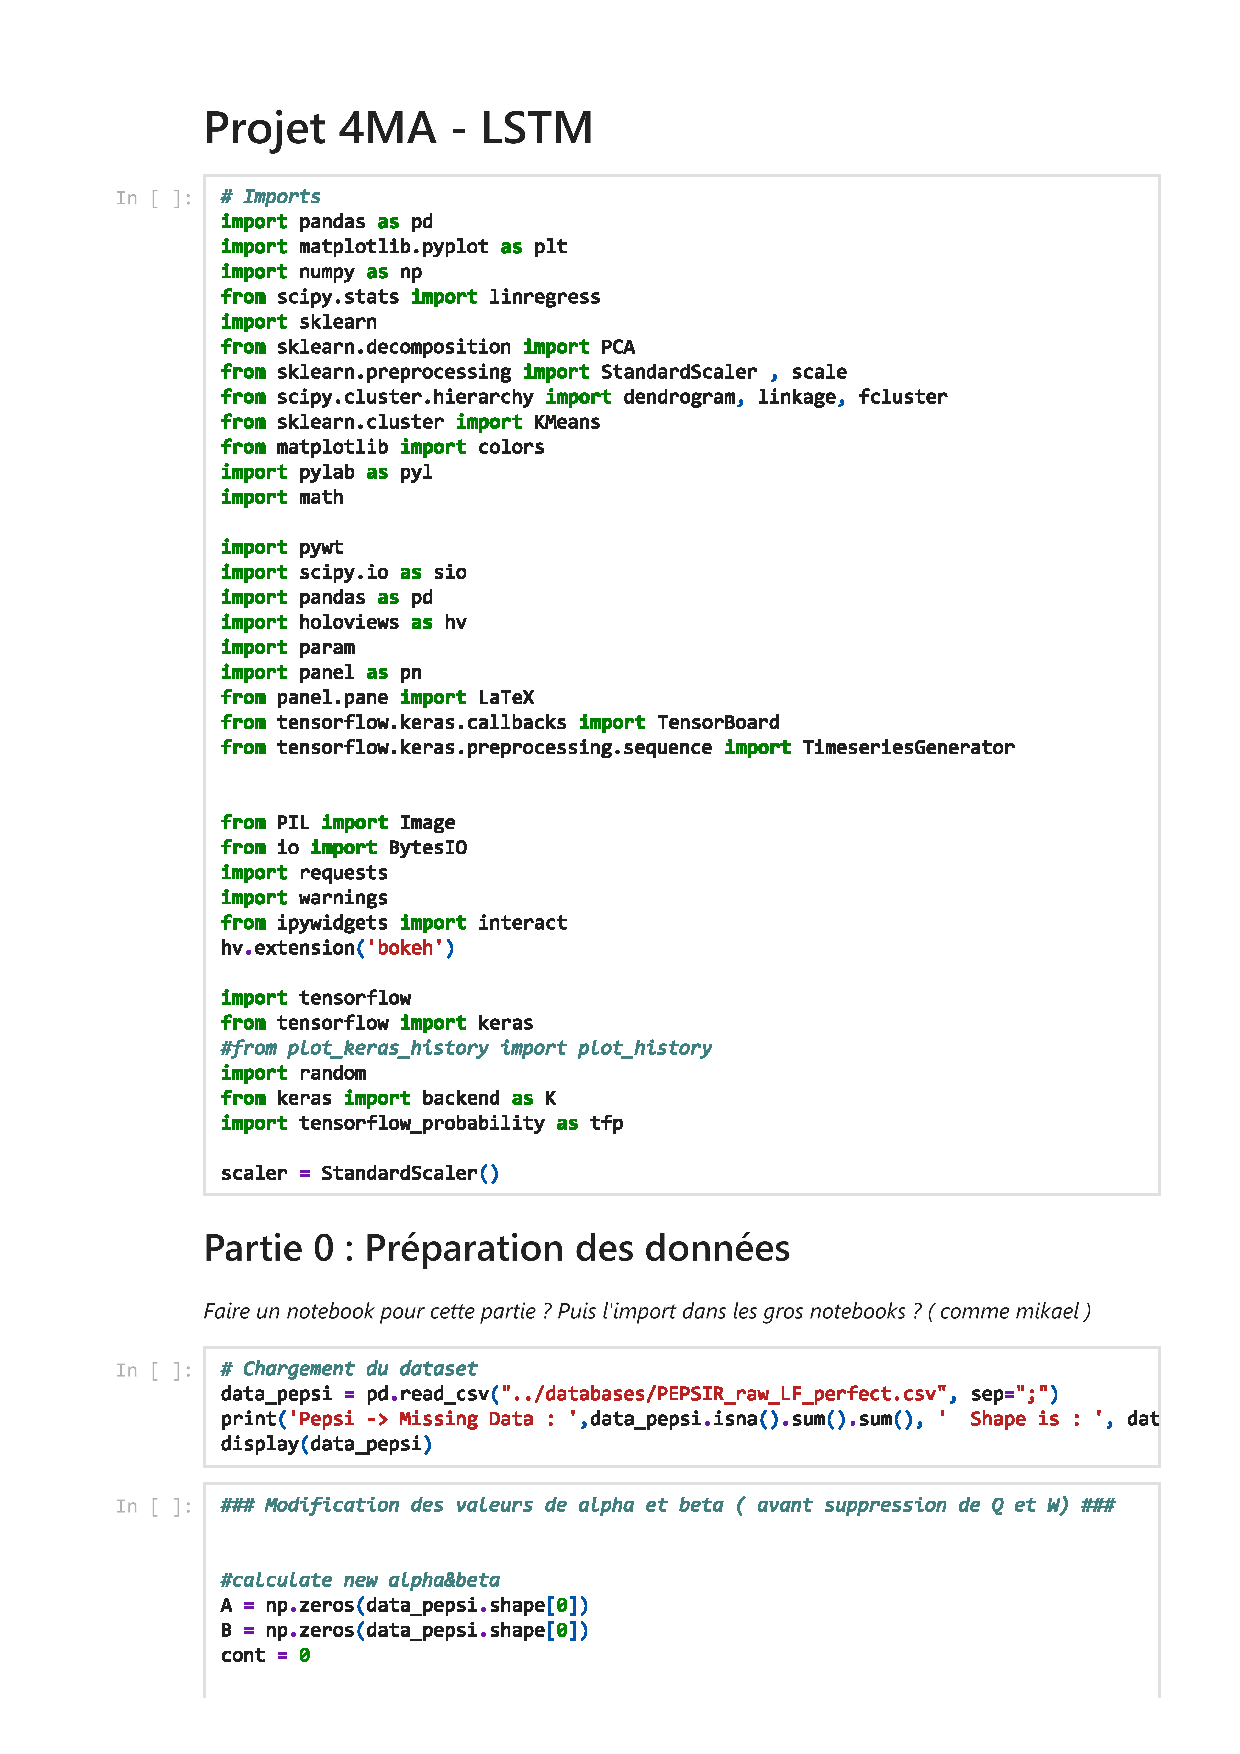
\includepdf[scale=0.7,pages=1, pagecommand=\section{Annex}]{pdf_lstm.pdf}
% \includepdf[scale=1,pages=2-]{pdf_lstm.pdf}
\end{document}